\documentclass[aspectratio=169,10pt]{beamer}

\usepackage{array}
\usepackage{booktabs}
\usepackage{graphicx}
\usepackage{amsmath}
\usepackage{amssymb}
\usepackage{tikz}
\usetikzlibrary{arrows.meta,calc,positioning,shapes.geometric,fit}
\newcolumntype{L}[1]{>{\raggedright\arraybackslash}p{#1}}

% DGIST ISL Custom Color Palette
\definecolor{islteal}{RGB}{43,133,147}
\definecolor{islred}{RGB}{203,76,65}
\definecolor{isldark}{RGB}{52,61,67}
\definecolor{islnavy}{RGB}{31,55,95}
\definecolor{islmuted}{RGB}{92,101,108}
\definecolor{isllight}{RGB}{236,241,243}
\definecolor{islgold}{RGB}{184,119,20}
\definecolor{islgreen}{RGB}{44,145,91}
\definecolor{islpurple}{RGB}{130,58,160}

\newcommand{\deckdate}{2026.08.21}
\newcommand{\labname}{DGIST Intelligent Systems and Learning Laboratory}

\setbeamersize{text margin left=0.65cm,text margin right=0.65cm}
\setbeamertemplate{navigation symbols}{}
\setbeamertemplate{blocks}[rounded][shadow=false]
\setbeamercolor{normal text}{fg=isldark,bg=white}
\setbeamercolor{frametitle}{fg=isldark,bg=white}
\setbeamercolor{footer}{fg=white,bg=isldark}
\setbeamerfont{frametitle}{series=\bfseries,size=\Large}
\setbeamerfont{normal text}{size=\small}

\setbeamertemplate{frametitle}{%
  \nointerlineskip%
  \begin{beamercolorbox}[wd=\paperwidth,ht=1.35cm,dp=0cm]{frametitle}
    \vskip0.45cm%
    \hspace*{0.74cm}\insertframetitle\par%
    \vskip0.05cm%
    \hspace*{0.74cm}{\color{islteal}\rule{0.68\paperwidth}{4pt}}%
    {\color{islred}\rule{0.20\paperwidth}{4pt}}%
  \end{beamercolorbox}%
}

\setbeamertemplate{footline}{%
  \leavevmode%
  \begin{beamercolorbox}[wd=\paperwidth,ht=0.34cm,dp=0.11cm]{footer}
    \hspace*{0.65cm}{\scriptsize\deckdate}%
    \hfill{\scriptsize Reinforcement Learning \& Robotics Track \quad $\vert$ \quad Week 02: Tabular Q-Learning}\hfill%
    {\scriptsize\insertframenumber\,/\,\inserttotalframenumber}\hspace*{0.65cm}%
  \end{beamercolorbox}%
}

\newcommand{\bottomrulebar}{%
  \begin{tikzpicture}[remember picture,overlay]
    \fill[islteal] (current page.south west) rectangle ++(0.43\paperwidth,0.11cm);
    \fill[isldark] ([xshift=0.43\paperwidth]current page.south west)
      rectangle ++(0.34\paperwidth,0.11cm);
    \fill[islred] ([xshift=0.77\paperwidth]current page.south west)
      rectangle ++(0.23\paperwidth,0.11cm);
  \end{tikzpicture}%
}

\newcommand{\sectionlabel}[1]{%
  {\small\bfseries\color{islteal}#1}\par\vspace{0.14cm}%
}

\begin{document}

% ==========================================
% SLIDE 1: Title Slide
% ==========================================
\begin{frame}[plain,noframenumbering]
  \bottomrulebar
  \vspace{1.00cm}
  {\centering
    {\fontsize{22}{26}\selectfont\bfseries\color{islnavy}
      Week 02: Tabular Q-Learning\par}
    \vspace{0.22cm}
    {\fontsize{15}{18}\selectfont\color{islteal}
      Discovering Optimal Action-Values from Experience\par}
    \vspace{0.50cm}
    {\large\bfseries Reinforcement Learning \& Robot Learning Core Curriculum\par}
    \vspace{0.20cm}
    {\small Presented by \textbf{DGIST ISL Team}\par}
    \vspace{0.12cm}
    {\small\color{islmuted} \labname\par}
    \vspace{0.10cm}
    {\small \deckdate\par}
    \vspace{0.45cm}
    {\scriptsize\color{islmuted}
      Core Concepts: Q-Table $\cdot$ Temporal-Difference Error $\cdot$ Bellman Optimality $\cdot$ $\epsilon$-Greedy Policy\par}
  }
\end{frame}

% ==========================================
% SLIDE 2: What is a Q-Table?
% ==========================================
\begin{frame}{From Domain Heuristics to Value Discovery}
  \sectionlabel{Can an agent autonomously discover optimal policies without human priors?}

  {\centering
    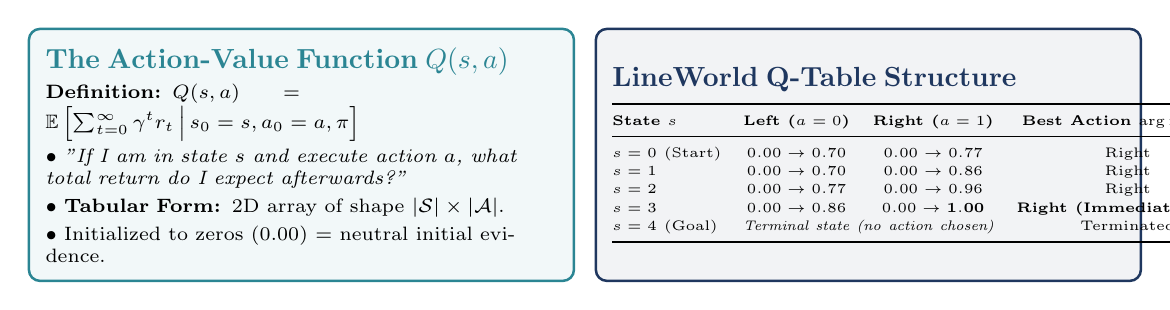
\begin{tikzpicture}[
      box/.style={rounded corners=4pt, text width=6.5cm, minimum height=3.2cm, inner sep=6pt, font=\scriptsize, line width=0.9pt, align=left}
    ]
      % Left Card: Meaning of Q
      \node[box, draw=islteal, fill=islteal!6] at (3.5, 1.7) {
        {\bfseries\color{islteal}\normalsize The Action-Value Function $Q(s, a)$}\\[3pt]
        \textbf{Definition:} $Q(s, a) = \mathbb{E}\left[ \sum_{t=0}^\infty \gamma^t r_t \,\Big|\, s_0=s, a_0=a, \pi \right]$\\[2pt]
        $\bullet$ \textit{"If I am in state $s$ and execute action $a$, what total return do I expect afterwards?"}\\[2pt]
        $\bullet$ \textbf{Tabular Form:} 2D array of shape $|\mathcal{S}| \times |\mathcal{A}|$.\\[2pt]
        $\bullet$ Initialized to zeros ($0.00$) = neutral initial evidence.
      };

      % Right Card: LineWorld Table
      \node[box, draw=islnavy, fill=islnavy!6] at (10.7, 1.7) {
        {\bfseries\color{islnavy}\normalsize LineWorld Q-Table Structure}\\[3pt]
        \renewcommand{\arraystretch}{1.1}
        \setlength{\tabcolsep}{4pt}
        {\centering
          \tiny
          \begin{tabular}{@{}lccc@{}}
            \toprule
            \textbf{State $s$} & \textbf{Left ($a=0$)} & \textbf{Right ($a=1$)} & \textbf{Best Action $\arg\max_a Q$} \\
            \midrule
            $s=0$ (Start) & $0.00 \to 0.70$ & $0.00 \to 0.77$ & Right \\
            $s=1$ & $0.00 \to 0.70$ & $0.00 \to 0.86$ & Right \\
            $s=2$ & $0.00 \to 0.77$ & $0.00 \to 0.96$ & Right \\
            $s=3$ & $0.00 \to 0.86$ & $0.00 \to \mathbf{1.00}$ & \textbf{Right (Immediate Goal)} \\
            $s=4$ (Goal) & \multicolumn{2}{c}{\textit{Terminal state (no action chosen)}} & Terminated \\
            \bottomrule
          \end{tabular}
        \par}
      };
    \end{tikzpicture}
  \par}
\end{frame}

% ==========================================
% SLIDE 3: The Temporal-Difference (TD) Mechanism
% ==========================================
\begin{frame}{The Temporal-Difference (TD) Learning Mechanism}
  \sectionlabel{Bootstrapping: updating an estimate from an immediate reward and an existing future guess}

  {\centering
    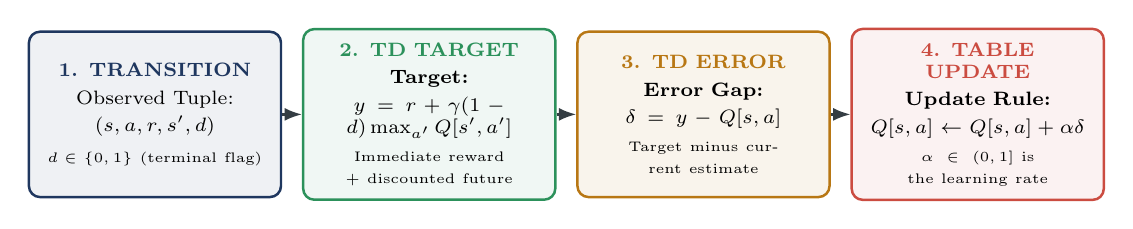
\begin{tikzpicture}[
      node distance=0.25cm,
      stage/.style={rounded corners=4pt, text width=2.85cm, minimum height=2.1cm, align=center, inner sep=5pt, font=\scriptsize, line width=0.9pt},
      arr/.style={-{Latex[length=2.2mm]}, thick, color=isldark}
    ]
      \node[stage, draw=islnavy, fill=islnavy!7] (trans) {
        {\bfseries\color{islnavy} 1. TRANSITION}\\[2pt]
        Observed Tuple:\\[2pt]
        $(s, a, r, s', d)$\\[3pt]
        \tiny $d \in \{0, 1\}$ (terminal flag)
      };

      \node[stage, draw=islgreen, fill=islgreen!7, right=of trans] (target) {
        {\bfseries\color{islgreen} 2. TD TARGET}\\[2pt]
        \textbf{Target:}\\[2pt]
        $y = r + \gamma(1-d)\max_{a'} Q[s', a']$\\[2pt]
        \tiny Immediate reward + discounted future
      };

      \node[stage, draw=islgold, fill=islgold!8, right=of target] (error) {
        {\bfseries\color{islgold} 3. TD ERROR}\\[2pt]
        \textbf{Error Gap:}\\[2pt]
        $\delta = y - Q[s, a]$\\[2pt]
        \tiny Target minus current estimate
      };

      \node[stage, draw=islred, fill=islred!7, right=of error] (update) {
        {\bfseries\color{islred} 4. TABLE UPDATE}\\[2pt]
        \textbf{Update Rule:}\\[2pt]
        $Q[s, a] \leftarrow Q[s, a] + \alpha \delta$\\[2pt]
        \tiny $\alpha \in (0, 1]$ is the learning rate
      };

      \draw[arr] (trans) -- (target);
      \draw[arr] (target) -- (error);
      \draw[arr] (error) -- (update);
    \end{tikzpicture}
  \par}

  \vspace{0.14cm}
  \begin{columns}[T,onlytextwidth]
    \column{0.48\textwidth}
      \begin{block}{\small\color{islteal}\textbf{Non-Terminal Case ($d=0$)}}
        \footnotesize Target $y = r + \gamma \max_{a'} Q[s', a']$. Value propagates backwards from goal one step at a time.
      \end{block}
    \column{0.48\textwidth}
      \begin{block}{\small\color{islred}\textbf{Terminal Case ($d=1$)}}
        \footnotesize Target $y = r$ at true task termination. An external time-limit truncation usually keeps the bootstrap term.
      \end{block}
  \end{columns}
\end{frame}

% ==========================================
% SLIDE 4: Hand Calculation Arithmetic
% ==========================================
\begin{frame}{Concrete Walkthrough: TD Arithmetic in LineWorld}
  \sectionlabel{Hand-traceable example: tracing values from initial state to goal ($(\alpha=0.5, \gamma=0.9)$)}

  {\centering
    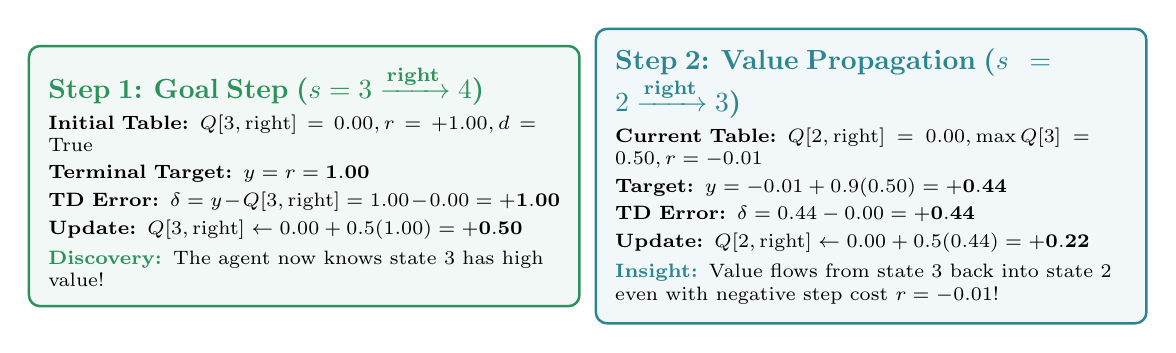
\begin{tikzpicture}[
      card/.style={rounded corners=4pt, text width=6.5cm, minimum height=3.3cm, align=left, inner sep=7pt, font=\scriptsize, line width=0.9pt}
    ]
      % Step A: Goal Step
      \node[card, draw=islgreen, fill=islgreen!6] at (3.5, 1.7) {
        {\bfseries\color{islgreen}\normalsize Step 1: Goal Step ($s=3 \xrightarrow{\text{right}} 4$)}\\[3pt]
        \textbf{Initial Table:} $Q[3, \text{right}] = 0.00, r=+1.00, d=\text{True}$\\[2pt]
        \textbf{Terminal Target:} $y = r = \mathbf{1.00}$\\[2pt]
        \textbf{TD Error:} $\delta = y - Q[3, \text{right}] = 1.00 - 0.00 = \mathbf{+1.00}$\\[2pt]
        \textbf{Update:} $Q[3, \text{right}] \leftarrow 0.00 + 0.5(1.00) = \mathbf{+0.50}$\\[3pt]
        {\color{islgreen}\bfseries Discovery:} The agent now knows state 3 has high value!
      };

      % Step B: Backpropagation Step
      \node[card, draw=islteal, fill=islteal!6] at (10.7, 1.7) {
        {\bfseries\color{islteal}\normalsize Step 2: Value Propagation ($s=2 \xrightarrow{\text{right}} 3$)}\\[3pt]
        \textbf{Current Table:} $Q[2, \text{right}] = 0.00, \max Q[3] = 0.50, r=-0.01$\\[2pt]
        \textbf{Target:} $y = -0.01 + 0.9(0.50) = \mathbf{+0.44}$\\[2pt]
        \textbf{TD Error:} $\delta = 0.44 - 0.00 = \mathbf{+0.44}$\\[2pt]
        \textbf{Update:} $Q[2, \text{right}] \leftarrow 0.00 + 0.5(0.44) = \mathbf{+0.22}$\\[3pt]
        {\color{islteal}\bfseries Insight:} Value flows from state 3 back into state 2 even with negative step cost $r=-0.01$!
      };
    \end{tikzpicture}
  \par}
\end{frame}

% ==========================================
% SLIDE 5: Exploration vs Exploitation
% ==========================================
\begin{frame}{Exploration vs. Exploitation: $\epsilon$-Greedy Policy}
  \sectionlabel{Balancing the discovery of new paths with the exploitation of known high-value actions}

  \begin{columns}[T,onlytextwidth]
    \column{0.48\textwidth}
      {\small\bfseries\color{islteal} The Dilemma}\par\vspace{0.08cm}
      {\footnotesize
      $\bullet$ \textbf{Pure Exploitation ($\epsilon=0$):} Always pick $\arg\max_a Q(s, a)$. May miss actions made unattractive by early estimates or tie-breaking.\\[2pt]
      $\bullet$ \textbf{Pure Exploration ($\epsilon=1$):} Random actions; does not deliberately exploit discovered paths.\\[3pt]}
      \begin{block}{\footnotesize $\epsilon$-Greedy Action Selection}
        $$a_t = \begin{cases} \text{random action} \in \mathcal{A}, & \text{with prob } \epsilon \\ \arg\max_a Q[s_t, a], & \text{with prob } 1 - \epsilon \end{cases}$$
      \end{block}

    \column{0.48\textwidth}
      {\small\bfseries\color{islnavy} Training vs Evaluation Discipline}\par\vspace{0.08cm}
      {\footnotesize
      $\bullet$ \textbf{During Training:} Use $\epsilon > 0$ (e.g. $\epsilon = 0.20$) so the agent discovers the entire state-action graph.\\[2pt]
      $\bullet$ \textbf{During Evaluation:} Set $\epsilon = 0$ (Pure Greedy).\\[2pt]
      $\bullet$ Evaluating with $\epsilon > 0$ injects artificial noise into policy benchmark metrics.\\[2pt]
      $\bullet$ Evaluate what the agent \textit{learned}, not how it explored!}
  \end{columns}
\end{frame}

% ==========================================
% SLIDE 6: Complete Tabular Q-Learning Algorithm
% ==========================================
\begin{frame}{System Architecture: The Tabular Q-Learning Loop}
  \sectionlabel{How exploration, environment feedback, and table updates form an autonomous learning loop}

  {\centering
    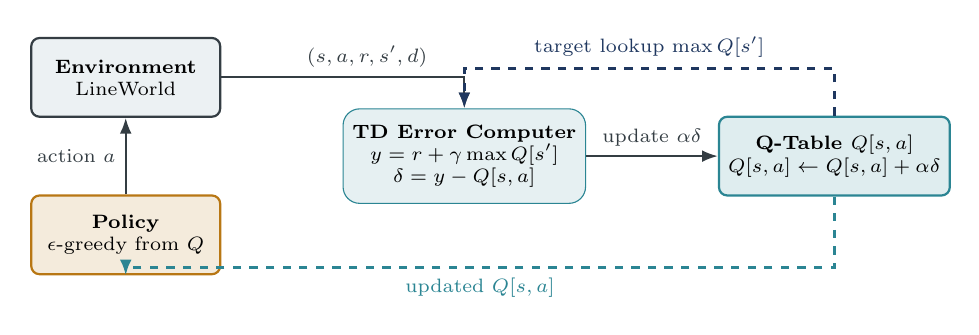
\begin{tikzpicture}[
      box/.style={rectangle, rounded corners=3pt, minimum width=2.4cm, minimum height=1.0cm, align=center, draw=isldark, line width=0.8pt, font=\scriptsize},
      data/.style={rectangle, rounded corners=6pt, draw=islteal, fill=islteal!12, minimum width=2.2cm, minimum height=1.2cm, font=\scriptsize, align=center},
      arr/.style={-{Latex[length=2.0mm]}, thick, color=isldark}
    ]
      % Env & Agent
      \node[box, fill=isllight] (env) at (1.5, 2.8) {\textbf{Environment}\\LineWorld};
      \node[box, fill=islgold!15, draw=islgold] (policy) at (1.5, 0.8) {\textbf{Policy}\\$\epsilon$-greedy from $Q$};

      % Center: TD Computer
      \node[data] (td) at (5.8, 1.8) {\textbf{TD Error Computer}\\$y = r + \gamma \max Q[s']$\\$\delta = y - Q[s, a]$};

      % Right: Q-Table
      \node[box, fill=islteal!15, draw=islteal, minimum width=2.8cm] (qtable) at (10.5, 1.8) {\textbf{Q-Table $Q[s, a]$}\\$Q[s, a] \leftarrow Q[s, a] + \alpha \delta$};

      % Forward & Feedback Loops
      \draw[arr] (policy) -- (env) node[midway, left]{\scriptsize action $a$};
      \draw[arr] (env) -| (td.north) node[pos=0.3, above]{\scriptsize $(s, a, r, s', d)$};
      \draw[arr] (td) -- (qtable) node[midway, above]{\scriptsize update $\alpha \delta$};
      \draw[arr, dashed, color=islteal, line width=1pt] (qtable.south) -- ++(0, -0.9) -| (policy.south) node[pos=0.25, below]{\scriptsize updated $Q[s, a]$};
      \draw[arr, dashed, color=islnavy, line width=1pt] (qtable.north) -- ++(0, 0.6) -| (td.north) node[pos=0.25, above]{\scriptsize target lookup $\max Q[s']$};
    \end{tikzpicture}
  \par}
\end{frame}

% ==========================================
% SLIDE 7: Code Lens - Examples Walkthrough
% ==========================================
\begin{frame}{Code Lens: Tabular Q-Learning in Python}
  \sectionlabel{Implementation patterns in examples/week-02}

  \begin{columns}[T,onlytextwidth]
    \column{0.50\textwidth}
      {\small\bfseries\color{islteal} Q-Table Data Structure}\par\vspace{0.06cm}
      {\footnotesize
      \begin{block}{\footnotesize Python 2D List}
\texttt{q\_table = [[0.0, 0.0] for \_ in range(5)]}\\[3pt]
\texttt{def update(s, a, r, s\_next, term):}\\
\texttt{\quad if term:}\\
\texttt{\quad\quad target = r}\\
\texttt{\quad else:}\\
\texttt{\quad\quad target = r + gamma * max(q\_table[s\_next])}\\
\texttt{\quad delta = target - q\_table[s][a]}\\
\texttt{\quad q\_table[s][a] += alpha * delta}
      \end{block}}

    \column{0.48\textwidth}
      {\small\bfseries\color{islgreen} Empirical Evaluation Benchmark}\par\vspace{0.06cm}
      \renewcommand{\arraystretch}{1.15}
      \setlength{\tabcolsep}{4pt}
      {\centering
        \footnotesize
        \begin{tabular}{@{}lcc@{}}
          \toprule
          \textbf{Policy} & \textbf{Avg Return} & \textbf{Success Rate} \\
          \midrule
          Random Policy & $+0.52$ & $65\%$ \\
          Always Right (Prior) & $+0.97$ & $100\%$ \\
          \textbf{Trained Q-Learner} & $\mathbf{+0.97}$ & $\mathbf{100\%}$ \\
          \bottomrule
        \end{tabular}
      \par}
      \vspace{0.14cm}
      \begin{alertblock}{\footnotesize What We Can Claim}
        Under this seed and evaluation protocol, Q-learning matched the known
        always-right reference without a hardcoded directional rule.
      \end{alertblock}
  \end{columns}
\end{frame}

% ==========================================
% SLIDE 8: Failure Modes & Debugging Traps
% ==========================================
\begin{frame}{Failure Modes in Tabular Q-Learning}
  \sectionlabel{Common conceptual and algorithmic pitfalls in tabular implementations}

  \begin{center}
    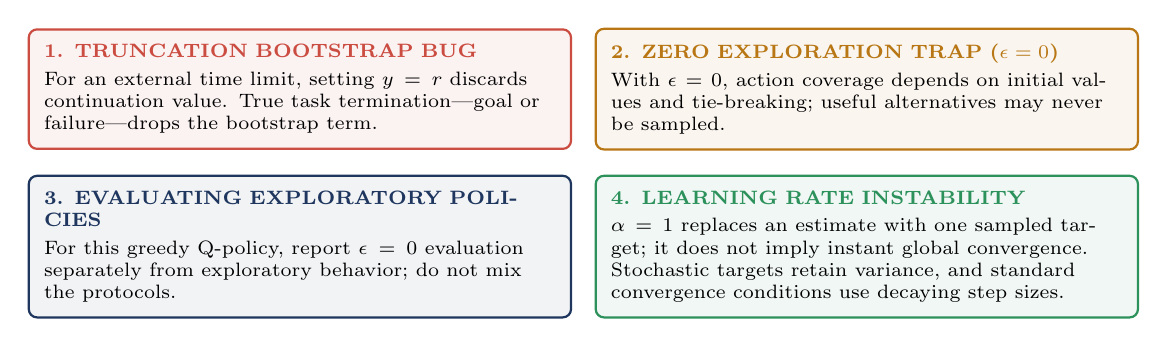
\begin{tikzpicture}[
      card/.style={rounded corners=3pt, text width=6.5cm, minimum height=1.35cm, align=left, inner sep=5.5pt, font=\scriptsize, line width=0.8pt}
    ]
      \node[card, draw=islred, fill=islred!7] at (3.5, 3.3) {
        {\bfseries\color{islred} 1. TRUNCATION BOOTSTRAP BUG}\\[2pt]
        For an external time limit, setting $y=r$ discards continuation value. True task termination---goal or failure---drops the bootstrap term.
      };

      \node[card, draw=islgold, fill=islgold!7] at (10.7, 3.3) {
        {\bfseries\color{islgold} 2. ZERO EXPLORATION TRAP ($\epsilon=0$)}\\[2pt]
        With $\epsilon=0$, action coverage depends on initial values and tie-breaking; useful alternatives may never be sampled.
      };

      \node[card, draw=islnavy, fill=islnavy!6] at (3.5, 1.3) {
        {\bfseries\color{islnavy} 3. EVALUATING EXPLORATORY POLICIES}\\[2pt]
        For this greedy Q-policy, report $\epsilon=0$ evaluation separately from exploratory behavior; do not mix the protocols.
      };

      \node[card, draw=islgreen, fill=islgreen!7] at (10.7, 1.3) {
        {\bfseries\color{islgreen} 4. LEARNING RATE INSTABILITY}\\[2pt]
        $\alpha=1$ replaces an estimate with one sampled target; it does not imply instant global convergence. Stochastic targets retain variance, and standard convergence conditions use decaying step sizes.
      };
    \end{tikzpicture}
  \end{center}
\end{frame}

% ==========================================
% SLIDE 9: Robotics Horizon Bridge
% ==========================================
\begin{frame}{Robotics Bridge: The Limits of Tabular Scaling}
  \sectionlabel{Why tabular lookups collapse on real physical robotic systems}

  \begin{columns}[T,onlytextwidth]
    \column{0.48\textwidth}
      {\small\bfseries\color{islnavy} The Curse of Dimensionality}\par\vspace{0.08cm}
      {\footnotesize
      $\bullet$ 7-DOF robot arm with joint angles discretized into 100 bins each:\\[2pt]
      $$\text{Table Rows} = 100^7 = 10^{14} \text{ discrete states!}$$\\[2pt]
      $\bullet$ Storing $10^{14}$ floats requires $\approx 800$ Terabytes of RAM.\\[2pt]
      $\bullet$ The robot would need millions of years of rollouts to visit every cell even once!}

    \column{0.48\textwidth}
      {\small\bfseries\color{islteal} The Bridge to Function Approximation}\par\vspace{0.08cm}
      {\footnotesize
      $\bullet$ Tabular cells do not generalize: visiting state $(1.000)$ gives zero knowledge about state $(1.001)$.\\[2pt]
      $\bullet$ \textbf{Parametric Approximation (Weeks 3--4):} Replace $Q[s, a]$ table with neural network $Q_\theta(s, a)$.\\[2pt]
      $\bullet$ Parameterized weights generalize value estimates across continuous physical state spaces.}
  \end{columns}
\end{frame}

% ==========================================
% SLIDE 10: Quiz Part 1 - Concepts Check
% ==========================================
\begin{frame}{Week 02 Quiz: Core Concepts \& Action-Values}
  \sectionlabel{Self-check: verify fundamental understanding of tabular Q-learning}

  \begin{center}
    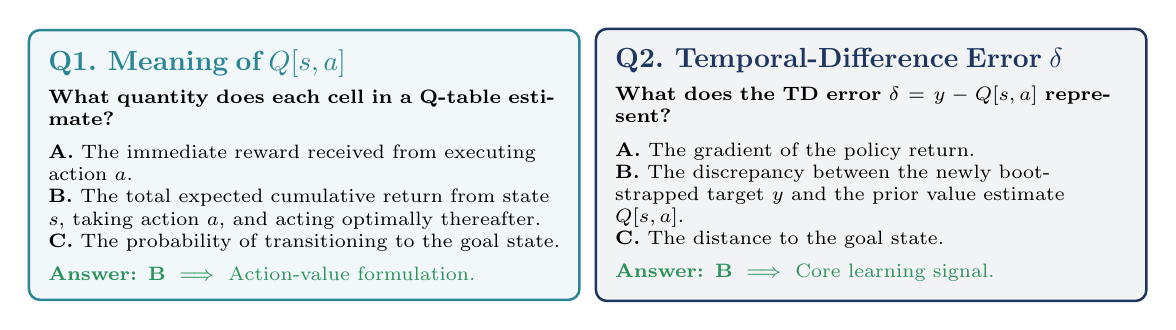
\begin{tikzpicture}[
      qcard/.style={rounded corners=4pt, text width=6.5cm, minimum height=3.3cm, align=left, inner sep=7pt, font=\scriptsize, line width=0.9pt}
    ]
      % Question 1
      \node[qcard, draw=islteal, fill=islteal!6] at (3.5, 1.7) {
        {\bfseries\color{islteal}\normalsize Q1. Meaning of $Q[s, a]$}\\[4pt]
        \textbf{What quantity does each cell in a Q-table estimate?}\\[4pt]
        \textbf{A.} The immediate reward received from executing action $a$.\\
        \textbf{B.} The total expected cumulative return from state $s$, taking action $a$, and acting optimally thereafter.\\
        \textbf{C.} The probability of transitioning to the goal state.
        \vskip4pt
        {\color{islgreen}\textbf{Answer: B} $\implies$ Action-value formulation.}
      };

      % Question 2
      \node[qcard, draw=islnavy, fill=islnavy!6] at (10.7, 1.7) {
        {\bfseries\color{islnavy}\normalsize Q2. Temporal-Difference Error $\delta$}\\[4pt]
        \textbf{What does the TD error $\delta = y - Q[s, a]$ represent?}\\[4pt]
        \textbf{A.} The gradient of the policy return.\\
        \textbf{B.} The discrepancy between the newly bootstrapped target $y$ and the prior value estimate $Q[s, a]$.\\
        \textbf{C.} The distance to the goal state.
        \vskip4pt
        {\color{islgreen}\textbf{Answer: B} $\implies$ Core learning signal.}
      };
    \end{tikzpicture}
  \end{center}
\end{frame}

% ==========================================
% SLIDE 11: Quiz Part 2 - TD Update Arithmetic
% ==========================================
\begin{frame}{Week 02 Quiz: TD Update Arithmetic}
  \sectionlabel{Verify hand-computations for tabular Q-learning updates}

  \begin{center}
    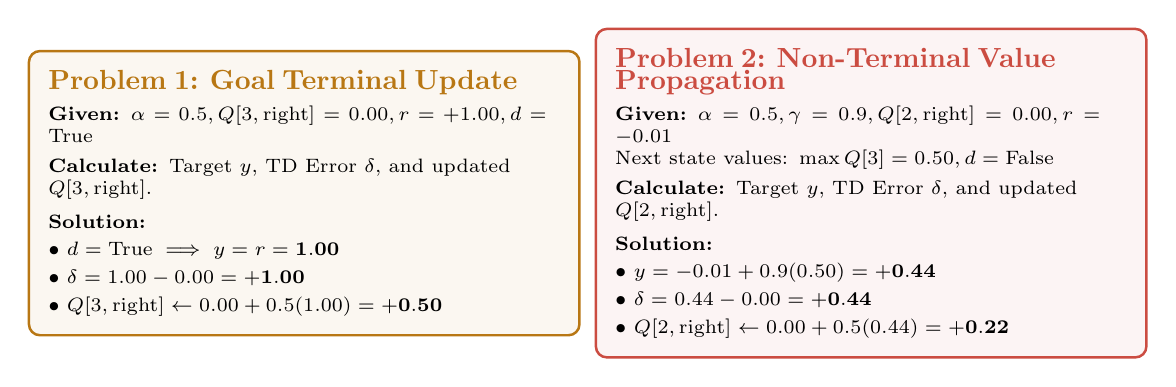
\begin{tikzpicture}[
      qcard/.style={rounded corners=4pt, text width=6.5cm, minimum height=3.3cm, align=left, inner sep=7pt, font=\scriptsize, line width=0.9pt}
    ]
      % Problem 1
      \node[qcard, draw=islgold, fill=islgold!6] at (3.5, 1.7) {
        {\bfseries\color{islgold}\normalsize Problem 1: Goal Terminal Update}\\[3pt]
        \textbf{Given:} $\alpha = 0.5, Q[3, \text{right}] = 0.00, r=+1.00, d=\text{True}$\\[3pt]
        \textbf{Calculate:} Target $y$, TD Error $\delta$, and updated $Q[3, \text{right}]$.\\[4pt]
        \textbf{Solution:}\\[2pt]
        $\bullet$ $d=\text{True} \implies y = r = \mathbf{1.00}$\\[2pt]
        $\bullet$ $\delta = 1.00 - 0.00 = \mathbf{+1.00}$\\[2pt]
        $\bullet$ $Q[3, \text{right}] \leftarrow 0.00 + 0.5(1.00) = \mathbf{+0.50}$
      };

      % Problem 2
      \node[qcard, draw=islred, fill=islred!6] at (10.7, 1.7) {
        {\bfseries\color{islred}\normalsize Problem 2: Non-Terminal Value Propagation}\\[3pt]
        \textbf{Given:} $\alpha = 0.5, \gamma = 0.9, Q[2, \text{right}] = 0.00, r=-0.01$\\
        Next state values: $\max Q[3] = 0.50, d=\text{False}$\\[3pt]
        \textbf{Calculate:} Target $y$, TD Error $\delta$, and updated $Q[2, \text{right}]$.\\[4pt]
        \textbf{Solution:}\\[2pt]
        $\bullet$ $y = -0.01 + 0.9(0.50) = \mathbf{+0.44}$\\[2pt]
        $\bullet$ $\delta = 0.44 - 0.00 = \mathbf{+0.44}$\\[2pt]
        $\bullet$ $Q[2, \text{right}] \leftarrow 0.00 + 0.5(0.44) = \mathbf{+0.22}$
      };
    \end{tikzpicture}
  \end{center}
\end{frame}

% ==========================================
% SLIDE 12: Quiz Part 3 - Interpretation & Traps
% ==========================================
\begin{frame}{Week 02 Quiz: Interpretation \& Practical Traps}
  \sectionlabel{Key practical questions every RL practitioner must master}

  \begin{center}
    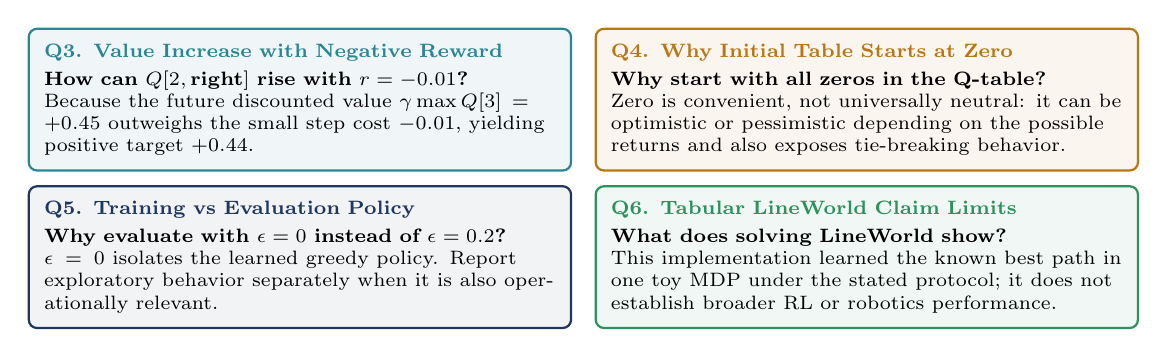
\begin{tikzpicture}[
      card/.style={rounded corners=3pt, text width=6.5cm, minimum height=1.35cm, align=left, inner sep=5.5pt, font=\scriptsize, line width=0.8pt}
    ]
      \node[card, draw=islteal, fill=islteal!7] at (3.5, 3.3) {
        {\bfseries\color{islteal} Q3. Value Increase with Negative Reward}\\[2pt]
        \textbf{How can $Q[2, \text{right}]$ rise with $r=-0.01$?}\\
        Because the future discounted value $\gamma \max Q[3] = +0.45$ outweighs the small step cost $-0.01$, yielding positive target $+0.44$.
      };

      \node[card, draw=islgold, fill=islgold!7] at (10.7, 3.3) {
        {\bfseries\color{islgold} Q4. Why Initial Table Starts at Zero}\\[2pt]
        \textbf{Why start with all zeros in the Q-table?}\\
        Zero is convenient, not universally neutral: it can be optimistic or pessimistic depending on the possible returns and also exposes tie-breaking behavior.
      };

      \node[card, draw=islnavy, fill=islnavy!6] at (3.5, 1.3) {
        {\bfseries\color{islnavy} Q5. Training vs Evaluation Policy}\\[2pt]
        \textbf{Why evaluate with $\epsilon=0$ instead of $\epsilon=0.2$?}\\
        $\epsilon=0$ isolates the learned greedy policy. Report exploratory behavior separately when it is also operationally relevant.
      };

      \node[card, draw=islgreen, fill=islgreen!7] at (10.7, 1.3) {
        {\bfseries\color{islgreen} Q6. Tabular LineWorld Claim Limits}\\[2pt]
        \textbf{What does solving LineWorld show?}\\
        This implementation learned the known best path in one toy MDP under the stated protocol; it does not establish broader RL or robotics performance.
      };
    \end{tikzpicture}
  \end{center}
\end{frame}

\end{document}
